% \iffalse
\let\negmedspace\undefined
\let\negthickspace\undefined
\documentclass[journal,12pt,twocolumn]{IEEEtran}
\usepackage{cite}
\usepackage{amsmath,amssymb,amsfonts,amsthm}
\usepackage{algorithmic}
\usepackage{graphicx}
\usepackage{textcomp}
\usepackage{xcolor}
\usepackage{txfonts}
\usepackage{listings}
\usepackage{enumitem}
\usepackage{mathtools}
\usepackage{gensymb}
\usepackage{comment}
\usepackage[breaklinks=true]{hyperref}
\usepackage{tkz-euclide} 
\usepackage{listings}
\usepackage{gvv}  
\usepackage{tikz}
\usepackage{circuitikz} 
\usepackage{caption}

\def\inputGnumericTable{}                                
\usepackage[latin1]{inputenc}                 
\usepackage{color}                            
\usepackage{array}                            
\usepackage{longtable}                        
\usepackage{calc}                            
\usepackage{multirow}                      
\usepackage{hhline}                           
\usepackage{ifthen}                          
\usepackage{lscape}
\usepackage{amsmath}
\newtheorem{theorem}{Theorem}[section]
\newtheorem{problem}{Problem}
\newtheorem{proposition}{Proposition}[section]
\newtheorem{lemma}{Lemma}[section]
\newtheorem{corollary}[theorem]{Corollary}
\newtheorem{example}{Example}[section]
\newtheorem{definition}[problem]{Definition}
\newcommand{\BEQA}{\begin{eqnarray}}
\newcommand{\EEQA}{\end{eqnarray}}
\newcommand{\define}{\stackrel{\triangle}{=}}
\theoremstyle{remark}
\newtheorem{rem}{Remark}

\begin{document}
\title{IIT HYDERABAD \\Arithmetic Progression Problem}
\author{Sasa Mardi, EE23BTECH11222}
\date{}
\maketitle
\textbf{Question 10.5.2-9:}
If the 3rd and the 9th terms of an AP are 4 and -8, respectively, which term of this AP is zero? \\
\solution
\begin{table}[h!]
    \centering
    \caption{Input Parameters}
    \label{tab:1}
    \begin{tabular}{ | c | c | c | }
        \hline
        Parameter & Value & Description \\
        \hline
        $T_3$ & 4 & Third term of the AP \\
        \hline
        $T_9$ & -8 & Ninth term of the AP \\
        \hline
         $x(n)$ & $x(0) + nd$ & $n^{th}$ term of the AP \\
        \hline
    \end{tabular}
\end{table}

From the values given in \tabref{tab:1}:
\begin{align}
    x(0) + 2d &= 4\\
    x(0) + 8d &= -8
\end{align}
On subtracting equation 1 from equation 2 :
\begin{align}
6d = -12 \\
d = -2 
\end{align}
Substitute d = -2 into:
\begin{align}
x(0) = 4 - 2d\\
x(0) = 4 - 2(-2) = 8
\end{align}
Substitute x(0) = 8 and d = -2 into:
\begin{align}
T_n = x(0) + (n-1)d = 0 \\
8 + (n-1)(-2) = 0 \\
n - 1 = 4 \\
n = 5
\end{align}
The term where the value is zero in the given arithmetic progression is the 5th term.\\
\begin{enumerate}
\item Finding $x(n)$ \\
The series is an arithmetic progression.
\begin{align}
x(n) = (x(0) + nd)(u(n))
\end{align}
as $x(n) = 0 \quad \forall \quad n < 0$.
\begin{figure}[h!]
    \centering
    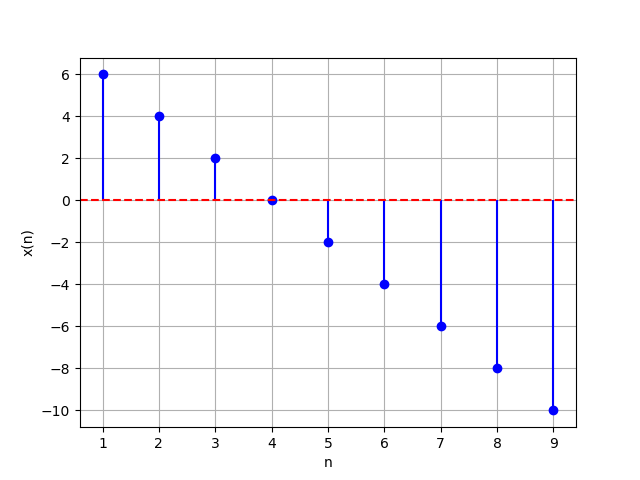
\includegraphics[width=\columnwidth]{xn.png}
    \caption{Plot of $x(n)$ vs $n$; Refer to \tabref{tab:1} for values of $x(0)$ and $d$}
    \label{fig:1}
\end{figure}
\item Z-transform of $x(n)$ \\
Let Z-transform of $x(n)$ be $X(z)$. Let $U(z)$ be the Z-transform of $u(n)$.
\begin{align}
X(z) &= \sum_{n = -\infty}^{\infty} (x(0) + nd)(u(n))(z^{-n}) \\
&= (x(0))(U(z)) + d\sum_{n = 0}^{\infty}nz^{-n} \\
&= (x(0))(U(z)) + d(\frac{z^{-1}}{(1 - z^{-1})^2}) \\
&= (x(0))(U(z)) + d(\frac{z}{(z - 1)^2}) \\
&= \frac{x(0)(z)}{z - 1} + \frac{dz}{(z - 1)^2} \quad \forall \quad |z| > 1
\end{align}
Using the values from \tabref{tab:1}:
\begin{align}
X(z) &= \frac{8z}{z - 1} + \frac{-2z}{(z - 1)^2} \quad \forall \quad |z| > 1
\end{align}
\end{enumerate}
\end{document}
